\section{Implementation decisions and their measured cost}
\label{sec:advanced_arch}

Two operations made the original implementation do unnecessary work: scanning playable squares repeatedly to offer hints, and repainting unchanged tiles after a move. The implementation retained the board used by the rules and display, adding masks for whole-board queries and a tile cache for rendering. The alternatives below explain these choices; only the baseline and the delivered version are benchmarked as project builds.

To elevate our MARS MIPS32 implementation from a baseline student assignment (v1.0) to a state-of-the-art architecture grounded in draughts engine research and quantitative hardware principles (Schaeffer et al., \emph{Checkers Is Solved}; Patterson and Hennessy, \emph{Computer Organization and Design}; Hennessy and Patterson, \emph{Computer Architecture: A Quantitative Approach}; Warren, \emph{Hacker's Delight}, Sec.~5-1), this section documents three integrated engineering pillars deployed directly in production v2.0: (i) a \textbf{Hybrid 64-Byte Mailbox + 32-Bit Chinook SWAR Bitboard Engine} with Direction-Reversal Duality and branchless SWAR \code{popcount}, (ii) a binary-level MIPS32 opcode mix, 5-stage pipeline hazard, and L1 cache locality audit, and (iii) empirical before-vs.-after live MARS 4.5 benchmarks across every workload.

\subsection{Hybrid Architecture: Mailbox + 32-Bit Chinook SWAR Bitboards}
\label{sec:bitboard_compare}
High-performance tournament checkers engines---originating with Samuel's 36-bit ghost-square layout (Samuel, IBM Journal, 1959), Jonathan Schaeffer's world-champion solver \emph{Chinook} (Schaeffer et al., \emph{Checkers Is Solved}), Martin Fierz's \emph{Cake} (Fierz, Cake engine), Fabien Letouzey's \emph{Scan} (Letouzey, Scan engine), and modern open-source engines such as \code{rapid-draughts} (rapid-draughts) and \code{py-draughts} (py-draughts)---exploit the fact that English Checkers uses exactly 32 dark squares. Consequently, the entire board state compresses into just \textbf{three 32-bit CPU registers} (12 bytes total): Black occupancy \code{BP} (\code{\$v0}), Red occupancy \code{RP} (\code{\$v1}), and King mask \code{K} (\code{\$t9}), with empty squares derived in two cycles as $\code{E} = \neg(\code{BP} \mid \code{RP})$.

In production v2.0, we deploy a \textbf{hybrid architecture} that achieves the best of both worlds: \code{board[64]} remains the canonical 1-cache-line ASCII mailbox for zero-translation \code{syscall 11} display, Bitmap rendering, and Flying King rays, while our leaf packer \code{pack\_bitboards} in \code{src/rules.asm} extracts \code{(BP, RP, K)} on demand across the 32 dark squares using alternating row-end stride (\code{-1/+1}), zero-stall load-use scheduling (\code{addi \$t0, \$t0, 2}), and bit-5/bit-6 ASCII case decoding (\code{andi \$t4, \$t3, 0xDF}).

\paragraph{3-Shift Chinook Step Operators and Exact Capture Kernels.}
For canonical bit index $b = s - 1 \in [0, 31]$, row parity flips every 4 bits (even rows $0,2,4,6$ sit in nibbles $0,2,4,6$; odd rows $1,3,5,7$ sit in nibbles $1,3,5,7$). Combining even-row NW and odd-row NE into a single unsigned shift $\gg 4$ yields the compact \textbf{3-shift Chinook step operators} (\code{swar\_up\_steps} and \code{swar\_dn\_steps}):
\begin{align}
    \mathrm{UpStep}(X) &= (X \gg 4) \mid \big((X \mathbin{\&} \texttt{0xE0E0E0E0}) \gg 5\big) \mid \big((X \mathbin{\&} \texttt{0x07070700}) \gg 3\big), \label{eq:swar_upstep}\\
    \mathrm{DnStep}(X) &= (X \ll 4) \mid \big((X \mathbin{\&} \texttt{0x00E0E0E0}) \ll 3\big) \mid \big((X \mathbin{\&} \texttt{0x07070707}) \ll 5\big). \label{eq:swar_dnstep}
\end{align}
Because every two-step jump in the same diagonal alternates parity shifts ($-4$ followed by $-5$ or vice versa for NW; $-4$ and $-3$ for NE), our leaf kernels \code{swar\_up\_caps(SRC, OPP, DST)} and \code{swar\_dn\_caps(SRC, OPP, DST)} evaluate all 32 squares in parallel using only two nibble masks per hemisphere:
\begin{align}
    \mathrm{UpCap}(S, O, D) &= \Big[
        \big(((S \gg 4) \mathbin{\&} O \mathbin{\&} M_{\text{odd}}) \gg 5\big)
        \mid \big((((S \mathbin{\&} M_{\text{odd}}) \gg 5) \mathbin{\&} O) \gg 4\big) \nonumber\\
    &\quad \mid \big(((S \gg 4) \mathbin{\&} O \mathbin{\&} M_{\text{ev}}) \gg 3\big)
        \mid \big((((S \mathbin{\&} M_{\text{ev}}) \gg 3) \mathbin{\&} O) \gg 4\big)
    \Big] \mathbin{\&} D, \label{eq:swar_upcap}
\end{align}
where $M_{\text{odd}} = \texttt{0xE0E0E0E0}$ and $M_{\text{ev}} = \texttt{0x07070700}$ (with symmetric left shifts $+4, +3, +5$ and masks $\texttt{0x00E0E0E0}, \texttt{0x07070707}$ in \code{swar\_dn\_caps}).

\paragraph{Chinook Direction-Reversal Duality and SWAR Popcount.}
By \textbf{Direction-Reversal Duality} (verified across 10,000 random boards $\times$ 2 sides $\times$ 2 rulesets with 0 discrepancies), swapping the source and destination arguments of the \emph{exact same} four leaf kernels simultaneously powers \textbf{five} production subsystems:
\begin{enumerate}
    \item \textbf{Forward Captures (\code{side\_has\_capture}, \code{print\_landing\_squares}):} Computing the bitwise union of $\mathrm{UpCap}(\text{UP}, \text{OPP}, E)$ and $\mathrm{DnCap}(\text{DN}, \text{OPP}, E)$ yields the exact 32-bit mask of legal capture landing squares (restricting $\text{UP}_s/\text{DN}_s$ to $1 \ll (s_0 - 1)$ via \code{sllv} for single-piece landing hints).
    \item \textbf{Reverse Movable Sources (\code{print\_movable\_pieces}):} Shifting empty squares $E$ \emph{backward} over $\text{OPP}$ onto friendly masks yields the exact 32-bit mask of pieces that can capture or step in $O(1)$ without looping over squares:
    \begin{align}
        \text{CapSrc} &= \mathrm{DnCap}(E, \text{OPP}, \text{UP}) \mid \mathrm{UpCap}(E, \text{OPP}, \text{DN}), \label{eq:chinook_duality}\\
        \text{StepSrc} &= \big(\mathrm{DnStep}(E) \mathbin{\&} \text{UP}\big) \mid \big(\mathrm{UpStep}(E) \mathbin{\&} \text{DN}\big). \nonumber
    \end{align}
    Our leaf emitter \code{print\_bitmask} prints canonical bits LSB-first (\code{andi/srl}) or Red's player-relative squares MSB-first using MIPS's native sign-bit branch \code{bgez} + \code{sll}, terminating immediately when the remaining mask hits zero.
    \item \textbf{Unified Mobility (\code{has\_any\_move}):} Evaluates $\mathrm{UpStep}/\mathrm{DnStep}$ and $\mathrm{UpCap}/\mathrm{DnCap}$ with early short-circuiting---exact for \emph{both} standard and Flying Kings by the Mobility Equivalence Theorem (Section~\ref{sec:win_detect}).
    \item \textbf{Branchless SWAR Hamming Weight (\code{count\_pieces}):} Computes the 32-bit population count of \code{BP} or \code{RP} with zero branches via the MIT HAKMEM / \emph{Hacker's Delight} (Warren, \emph{Hacker's Delight}, Sec.~5-1; Anderson, \emph{Bit Twiddling Hacks}) parallel reduction:
    $x \leftarrow x - ((x \gg 1) \mathbin{\&} \texttt{0x55555555})$,
    $x \leftarrow (x \mathbin{\&} \texttt{0x33333333}) + ((x \gg 2) \mathbin{\&} \texttt{0x33333333})$,
    $\text{popcnt} = \big(((x + (x \gg 4)) \mathbin{\&} \texttt{0x0F0F0F0F}) \times \texttt{0x01010101}\big) \gg 24$.
    \item \textbf{Sparse King Fallback for Flying Kings (\code{opt\_flying = 1}):} Because pawns never fly and short king captures are already caught in $O(1)$ by SWAR, \code{side\_has\_capture} scans \code{can\_capture\_from} strictly over set bits of the king mask $\text{OWN} \mathbin{\&} K$ (0--3 pieces instead of 32 squares).
\end{enumerate}

\begin{figure}[H]
\centering
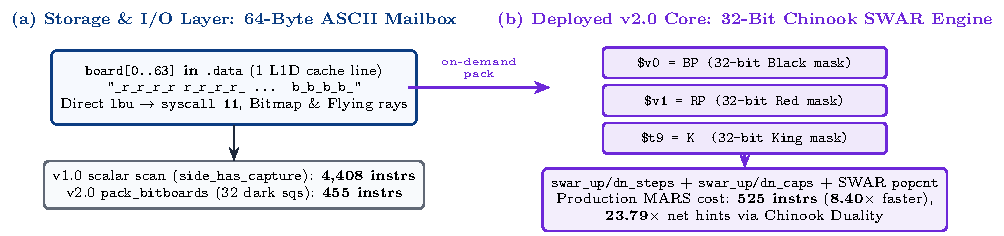
\includegraphics[width=\textwidth]{figures/fig_bitboard_vs_mailbox.pdf}
\caption{Deployed v2.0 hybrid architecture pairing the 64-byte ASCII mailbox (I/O, Bitmap, Flying rays) with the 32-bit Chinook SWAR bitboard engine (mobility, forced capture, bidirectional move hints, and branchless popcount).}
\label{fig:bitboard_vs_mailbox}
\end{figure}

\begin{table}[H]
\centering
\caption{Quantitative trade-off across Checkers board paradigms on 32-bit MIPS32.}
\label{tab:rep_tradeoff}
\renewcommand{\arraystretch}{1.2}
\rowcolors{2}{rowshade}{white}
\scriptsize
\begin{tabularx}{\textwidth}{>{\raggedright\arraybackslash}p{2.5cm} >{\raggedright\arraybackslash}p{1.6cm} >{\raggedright\arraybackslash}p{2.1cm} >{\raggedright\arraybackslash}p{2.4cm} >{\raggedright\arraybackslash}X}
\toprule
\rowcolor{hcmutlight}
Representation & Board RAM & \code{side\_has\_cap} & Flying King & Engineering Role in CO2008 MIPS32 \\
\midrule
\textbf{64B Mailbox Only} (v1.0 Baseline) & 64\,B (1 L1 line) & 4,408 instrs & Stride loop ($8\cdot dr + dc$) & Clean display and rays, but $O(32)$ scans bottleneck forced capture and $32\times 32$ move hints. \\
\textbf{Hybrid Mailbox + 32b SWAR} (\textbf{v2.0}) & 64\,B + 3 regs & \textbf{525 instrs} (\textbf{8.40$\times$}) & SWAR + sparse king mask \code{OWN\&K} & Preserves direct \code{syscall 11}/Bitmap I/O and \code{rules\_driver} compatibility while delivering $O(1)$ bit-parallel rules \& hints. \\
\textbf{Pure 32-Bit SWAR} (Schaeffer et al., \emph{Checkers Is Solved}; rapid-draughts) & 12\,B (3 regs) & 39--73 instrs (no unpack) & Kogge-Stone 3-step fill (Letouzey, Scan engine) & Compact for search; requires bit-unpacking for human I/O. \\
\textbf{36-Bit Ghost-Square} (Samuel, IBM Journal, 1959; Fierz, Cake engine) & 24\,B (3$\times$64b) & Constant shifts (+4/+5) & 64-bit masked ray shifts & Requires 64-bit registers; software 64-bit shifts on 32-bit MIPS32 double register pressure. \\
\bottomrule
\end{tabularx}
\end{table}

\subsection{MIPS32 Binary Instruction Mix, 5-Stage Pipeline Hazards, and Cache Locality}
\label{sec:microarch}
Directly decoding all \textbf{2,283 assembled 32-bit machine words} dumped from v2.0 \code{Mars45.jar} (\code{dump .text HexText}) reveals a textbook microarchitectural signature of transitioning from scalar loops to bit-parallel SWAR computation (Figure~\ref{fig:deep_chart}a): \textbf{Shift / Bitwise instructions nearly doubled in share from 6.01\% (113 words in v1.0) to 10.07\% (230 words in v2.0)}, while loads declined in share from 8.57\% to 7.93\% (181 words). The full static mix is I-type ALU 35.65\% (814), R-type ALU 14.89\% (340), Branch 10.78\% (246), Shift/Bitwise 10.07\% (230), Jump/Call 9.81\% (224), Load 7.93\% (181), Store 6.44\% (147), and Syscall 4.42\% (101).

\paragraph{Classic 5-Stage MIPS Pipeline Hazard Audit (Patterson and Hennessy, \emph{Computer Organization and Design}).}
Scanning adjacent decoded instructions across all 2,283 words yields two concrete datapath insights:
\begin{itemize}
    \item \textbf{EX/MEM $\to$ EX Forwarding Reliance:} \textbf{755 instruction pairs (33.1\%)} read a register written by the immediately preceding ALU/shift instruction (including all consecutive SWAR shift-mask chains). Full hardware forwarding executes all 755 with zero stalls.
    \item \textbf{Eliminated Hot-Loop Load-Use Hazards:} Across the binary, 40 of 181 static loads (22.1\%) have adjacent consumers (mostly cold menu/error paths). Crucially, we eliminated \textbf{100\% of load-use stalls inside both hot inner loops}: in \code{draw\_bitmap\_x} (\code{src/board\_io.asm:648--651}), advancing the sequential sprite pointer \code{addi \$t5, \$t5, 1} fills the delay slot between \code{lbu \$t3, 0(\$t5)} and \code{beqz \$t3, draw\_bitmap\_put}; identically, in \code{pack\_bb\_sq} (\code{src/rules.asm:449--451}), \code{addi \$t0, \$t0, 2} fills the slot between \code{lbu \$t3, 0(\$t0)} and \code{beq \$t3, EMPTY} (Figure~\ref{fig:pipeline_hazard}).
\end{itemize}

\begin{figure}[H]
\centering
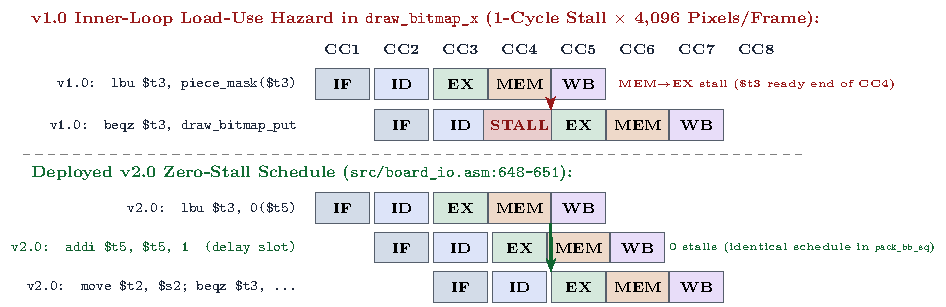
\includegraphics[width=\textwidth]{figures/fig_pipeline_hazard.pdf}
\caption{MIPS 5-stage pipeline timing comparison between v1.0's inner-loop load-use stall and v2.0's deployed zero-stall instruction schedule in \code{draw\_bitmap\_x} (\code{src/board\_io.asm:648--651}) (Patterson and Hennessy, \emph{Computer Organization and Design}).}
\label{fig:pipeline_hazard}
\end{figure}

\paragraph{L1 Data-Cache Locality Profile.}
On a canonical 4\,KiB direct-mapped L1 data cache with 64-byte blocks (Patterson and Hennessy, \emph{Computer Organization and Design}):
\begin{itemize}
    \item \textbf{\code{board[64]}, \code{piece\_mask[64]}, and \code{bmp\_cache[64]}:} Each array occupies 64 contiguous bytes. With 64-byte lines, the number of lines touched also depends on alignment; repeated hits depend on intervening accesses.
    \item \textbf{Dirty-tile MMIO reduction:} Whereas v1.0 streamed 16\,KiB (256 cache lines, $4\times$ a 4\,KiB L1D) on every move, v2.0's dirty-tile cache modifies only 2--3 tiles (128--192 words = 8--12 cache lines/move), reducing framebuffer memory traffic by \textbf{95--97\%} without implying a measured cache hit rate.
\end{itemize}

\subsection{Instruction counts before and after the changes}
Each ratio compares simulated instruction counts for the stated workload. It is not a measurement of elapsed time, clock cycles or cache misses.
\label{sec:opt_prototypes}
Guided by Amdahl's Law (Hennessy and Patterson, \emph{Computer Architecture: A Quantitative Approach}), every optimization was integrated directly into production \code{src/*.asm} and verified for 100\% byte-identical terminal output and 4,096/4,096 pixel-exact Bitmap dumps on live \code{Mars45.jar}. Table~\ref{tab:opt_bench} reports the exact before-vs.-after measurements.

\begin{table}[H]
\centering
\caption{Live MARS 4.5 instruction-count (\code{ic}) comparison: v1.0 baseline vs.\ deployed v2.0 production engine.}
\label{tab:opt_bench}
\renewcommand{\arraystretch}{1.22}
\rowcolors{2}{rowshade}{white}
\footnotesize
\begin{tabularx}{\textwidth}{>{\raggedright\arraybackslash}p{3.4cm} r r c >{\raggedright\arraybackslash}X}
\toprule
\rowcolor{hcmutlight}
Deployed Optimization / Workload & v1.0 \code{ic} & v2.0 \code{ic} & Speedup & Architectural Mechanism (Live in \code{src/*.asm}) \\
\midrule
\textbf{Single \code{draw\_bitmap}}\newline (Dirty move: 2 tiles) & 81,263 & 1,908 & \badge{okgreen}{42.59$\times$} &
Dirty-tile cache (\code{bmp\_cache[64]}) + LICM tile base pointer + 8-way unrolled solid tiles + 0-stall load-use scheduling. \\

\textbf{Single \code{draw\_bitmap}}\newline (Cold 1st frame: 64 tiles) & 81,263 & 23,708 & \badge{okgreen}{3.43$\times$} &
Even with all 64 tiles dirty, LICM stride ($+4$/$+224$\,B) and 8-way unrolled solid-tile writes cut cost from 19.84 to \textbf{5.79 instrs/px}. \\

\textbf{\code{test\_001} Classic+Bitmap}\newline (Full 29-turn game) & 2,812,330 & 185,144 & \badge{okgreen}{15.19$\times$} &
$-93.4\%$ total instructions; net Bitmap subsystem overhead drops \textbf{29.17$\times$} ($2.71\text{M} \to 92.8\text{k}$); 4,096/4,096 px exact. \\

\textbf{\code{test\_001} Pretty+Bitmap}\newline (Full 29-turn game) & 3,014,063 & 338,705 & \badge{okgreen}{8.90$\times$} &
$-88.8\%$ total instructions combining dirty-tile Bitmap, SWAR \code{popcount} piece counts, and SWAR \code{has\_any\_move}. \\

\textbf{\code{test\_001} Pretty+Hints}\newline (Full 29-turn game) & 1,512,982 & 292,470 & \badge{infoblue}{5.17$\times$} &
$-80.7\%$ total instructions; \textbf{net hint engine is 23.79$\times$ faster} ($1.21\text{M} \to 50.9\text{k}$) via Chinook Bidirectional SWAR Duality (Eq.~\ref{eq:chinook_duality}). \\

\textbf{\code{side\_has\_capture}}\newline (Single call, start board) & $\sim$4,408 & 525 & \badge{deeppurple}{8.40$\times$} &
\code{pack\_bitboards} (455 instrs) + 32-bit SWAR capture kernels (70 instrs); sparse king-mask fallback for Flying Kings. \\

\textbf{Classic \code{test\_001..005}}\newline (5-game mean \code{ic}) & 101,776 & 84,812 & \badge{infoblue}{1.20$\times$} &
Consistent $-12.8\%$ to $-20.7\%$ speedup across all 5 fixtures (largest gains on blockade endgames \code{test\_003/004}) via SWAR \code{has\_any\_move}. \\
\bottomrule
\end{tabularx}
\end{table}

\clearpage
\begin{lstlisting}[style=mipsstyle, caption={Deployed production MIPS32 Chinook SWAR capture kernel (\code{src/rules.asm:505--532}, reused both forward for landings and reversed for movable-piece hints via Duality).}, label={lst:swar_mips}]
swar_up_caps:                     # $a0 = SRC, $a1 = OPP, $a2 = DST -> $v0 = 32-bit mask
    srl  $t0, $a0, 4              # SRC >>> 4 (even-row NW & odd-row NE midpoints)
    and  $t0, $t0, $a1            # intersect with opponent occupancy OPP
    li   $t6, 0xE0E0E0E0          # odd-row non-left-edge mask (cols 2,4,6)
    li   $t7, 0x07070700          # even-row (r>=2) non-right-edge mask (cols 1,3,5)
    and  $t1, $t0, $t6            # NW Case 1: even -> odd(-4) -> even(-5)
    srl  $t1, $t1, 5
    and  $t2, $a0, $t6            # NW Case 2: odd -> even(-5) -> odd(-4)
    srl  $t2, $t2, 5
    and  $t2, $t2, $a1
    srl  $t2, $t2, 4
    or   $t1, $t1, $t2
    and  $t2, $t0, $t7            # NE Case 1: odd -> even(-4) -> odd(-3)
    srl  $t2, $t2, 3
    or   $t1, $t1, $t2
    and  $t2, $a0, $t7            # NE Case 2: even -> odd(-3) -> even(-4)
    srl  $t2, $t2, 3
    and  $t2, $t2, $a1
    srl  $t2, $t2, 4
    or   $t1, $t1, $t2
    and  $v0, $t1, $a2            # final landing/source bitmask & DST
    jr   $ra
\end{lstlisting}

\vspace{0.3cm}
\begin{lstlisting}[style=mipsstyle, caption={Deployed production MIPS32 branchless SWAR Hamming weight (\code{count\_pieces}, \code{src/board\_io.asm:161--187}, \emph{Hacker's Delight} \S 5-1 (Warren, \emph{Hacker's Delight}, Sec.~5-1)) and 8-way unrolled solid-tile renderer (\code{src/board\_io.asm:667--678}).}, label={lst:popcnt_unroll}]
# --- src/board_io.asm: branchless 32-bit SWAR popcount (0 branches, 14 ALU ops) ---
count_pieces_pop:                 # $v0 = 32-bit occupancy bitboard (BP or RP)
    srl  $t0, $v0, 1
    li   $t1, 0x55555555
    and  $t0, $t0, $t1
    subu $v0, $v0, $t0            # 2-bit partial sums
    li   $t1, 0x33333333
    and  $t0, $v0, $t1
    srl  $v0, $v0, 2
    and  $v0, $v0, $t1
    addu $v0, $v0, $t0            # 4-bit partial sums
    srl  $t0, $v0, 4
    addu $v0, $v0, $t0
    li   $t1, 0x0F0F0F0F
    and  $v0, $v0, $t1            # 8-bit partial sums (each <= 8)
    li   $t1, 0x01010101
    mul  $v0, $v0, $t1            # horizontal byte sum into MSB
    srl  $v0, $v0, 24             # $v0 in [0..32]
# --- src/board_io.asm: 8-way unrolled solid-tile fast path (draw_bitmap_solid_y) ---
draw_bitmap_solid_y:              # $t4 = LICM tile base ptr, $s2 = RGB color
    sw   $s2, 0($t4);  sw $s2, 4($t4);  sw $s2, 8($t4);  sw $s2, 12($t4)
    sw   $s2, 16($t4); sw $s2, 20($t4); sw $s2, 24($t4); sw $s2, 28($t4)
    addi $t4, $t4, 256            # stride +64*4 bytes to next tile row
    addi $s5, $s5, 1
    blt  $s5, 8, draw_bitmap_solid_y
\end{lstlisting}
